% --- SIDE-BY-SIDE FIGURES (SHARING PAGE WIDTH) ---
\begin{figure*}[!t]
  \centering
  % Left Side: Dataset Samples
  \begin{minipage}{0.48\textwidth}
    \centering
    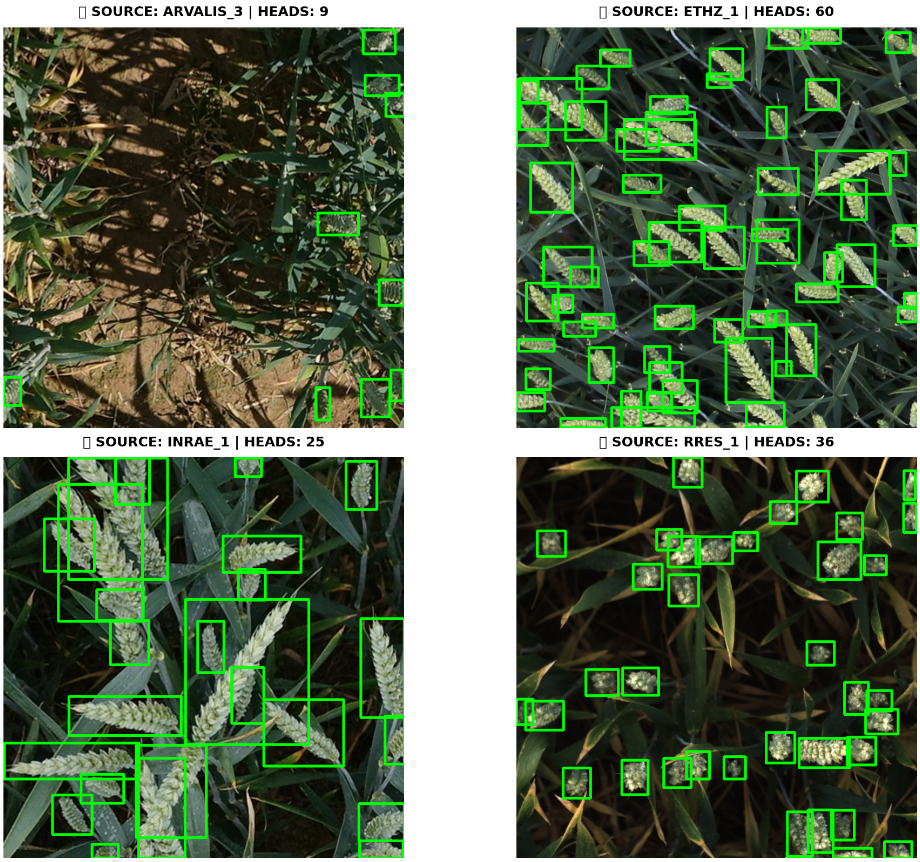
\includegraphics[width=\linewidth]{wheat_variance.png}
    \caption{Sample images from the GWHD demonstrating significant inter-domain variability. Clockwise from top left: sparse canopy (ARVALIS), high-density clustering (ETHZ), variable illumination (RRES), and phenotypic variance (INRAE).}
    \label{fig:dataset_variance}
  \end{minipage}
  \hfill % Adds space between the two images
  % Right Side: Architecture Diagram
  \begin{minipage}{0.48\textwidth}
    \centering
    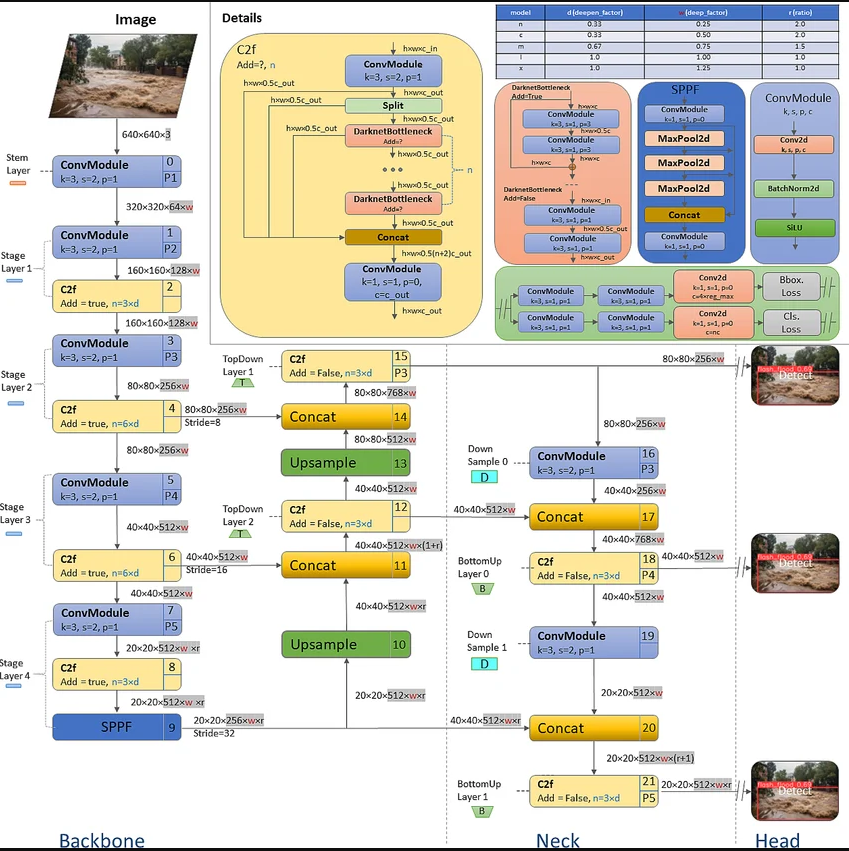
\includegraphics[width=\linewidth]{sec/yolov8s_1.png}
    \caption{Schematic representation of the YOLOv8s architecture, highlighting the CSPDarknet backbone, SPPF module, and decoupled anchor-free heads.}
    \label{fig:yolo_arch}
  \end{minipage}
\end{figure*}

\section{Proposed Methodology}
\label{sec:methodology}

To construct the AgriVision Decision Support System, we developed a deterministic pipeline that bridges pixel-level feature extraction with macro-level agronomic analytics. This section details the data preprocessing protocol, the theoretical framework of our selected detection architecture, and the mathematical formulation of our decision support engine.

\subsection{Data Pipeline and Preprocessing}
\label{subsec:data_prep}

The foundation of our detection architecture relies on robust feature extraction from highly variable agricultural imagery. 

\textbf{Dataset Characteristics and Provenance:} We utilized the Global Wheat Head Dataset (GWHD) 2020 \cite{ren2015faster}, acquired via the official CoDALab release. The dataset comprises 3,422 high-resolution ($1024 \times 1024$ pixels) images containing 145,411 dense bounding box annotations. A defining characteristic of the GWHD is its multi-institutional provenance; data was aggregated from seven independent research facilities across six countries.

This geographic diversity introduces profound inter-domain variability. The dataset exhibits significant variance in phenotypic morphology, illumination, and canopy density. EDA revealed a heavy-tailed distribution of bounding boxes per image ($\mu=42.5, \sigma \approx 20.1$), with outliers containing over 100 heavily occluded instances. These outliers were retained to train a robust, shape-dependent regression head.

\textbf{Source-Stratified Partitioning:} To prevent domain shift, we implemented a source-stratified splitting protocol. We partitioned the dataset into an 80/20 train/test split, stratified by the institutional source metadata. A subsequent 80/20 split on the training partition was performed at the \texttt{image\_id} level to generate the validation set, guaranteeing zero data leakage.

\textbf{Pipeline Validation via Faster R-CNN:} Prior to primary training, we instituted a software-engineering sanity check. A PyTorch-based Faster R-CNN \cite{ren2015faster} utilizing a ResNet-50-FPN backbone (pre-trained on MS COCO \cite{lin2014microsoft}) was deployed as a validation instrument. Monotonic loss convergence on a minimal CPU subset verified the integrity of the data ingestion and gradient flow.

\subsection{Architecture Selection: YOLOv8s}
\label{subsec:architecture}

For the primary detection task, we selected the YOLOv8 small (YOLOv8s) architecture. While transformer-based detectors offer high precision, their computational complexity makes them prohibitive for real-time agricultural deployment on UAV hardware. YOLOv8s strikes an optimal Pareto frontier between inference velocity and mAP.

The superiority of YOLOv8s for dense field detection stems from its anchor-free detection head. By decoupling classification and regression, the model directly predicts object centers, which is advantageous for dense, overlapping clusters in the GWHD. Furthermore, the Spatial Pyramid Pooling - Fast (SPPF) module (visualized in Figure~\ref{fig:yolo_arch}) ensures multi-scale feature awareness, allowing for the simultaneous detection of proximal and distal wheat heads.

